\documentclass[spanish]{thesis}

\author{Antonio Luis Farres Corzo}
\title{Sistema web para la evaluación de la Madurez Digital basado en la tecnología TETR4DIG-STD}
\ucicenter{Facultad de Tecnologías Interactivas}
\facultynum{4}
\addtutor{MSc. Ing. Noel Emilio Rojas Martos}

\thought{Escribe aquí tu pensamiento o frase inspiradora\\
 Autor del pensamiento}
 
\dedicatory{Escribe aquí tu dedicatoria}

\acknowledgment{Escribe aquí tus agradecimientos}

\abstract{La presente investigación aborda la necesidad de modernizar y automatizar el proceso de evaluación de la madurez digital en la Dirección de Consultoría de la Empresa de Telecomunicaciones de Cuba S.A. (ETECSA), integrando el marco conceptual de la tecnología TETR4DIG-STD en una plataforma tecnológica eficiente. El objetivo general consistió en desarrollar un sistema web integral bajo una arquitectura Fullstack que permitiera centralizar la captura de datos y la visualización de indicadores estratégicos. Metodológicamente, se empleó la metodología ágil Extreme Programming (XP), lo cual facilitó un desarrollo incremental y adaptativo mediante prácticas técnicas de calidad como las historias de usuario y entregas pequeñas. Para la implementación del servidor de aplicaciones se utilizó el framework Django con una base de datos centralizada, mientras que el lado del cliente fue construido con la biblioteca React, incorporando herramientas de visualización para la generación de reportes profesionales en tiempo real. Los principales hallazgos demostraron que la transición del método manual basado en hojas de cálculo hacia una solución web automatizada reduce significativamente la fragmentación de la información y el riesgo de errores en los diagnósticos. Como conclusión, el sistema desarrollado se consolidó como una herramienta estratégica que garantiza la integridad de los datos y optimiza la toma de decisiones informadas en el proceso de transformación organizacional de la entidad.}

\keywords{transformación digital, madurez digital, TETR4DIG-STD, Django, React, XP}

\input{Glossary}
\input{Acronyms}

\addbibresource{example.bib}

\begin{document}
  \maketitle
  
  \introduction

El panorama contemporáneo de las industrias creativas se caracteriza por una alta dependencia de activos digitales. Desde el diseño gráfico y la producción audiovisual hasta el desarrollo de videojuegos, la capacidad de crear, almacenar, localizar y reutilizar recursos digitales de forma eficiente constituye un factor crítico de productividad y competitividad. Sin embargo, la práctica profesional evidencia una gestión fragmentada de estos recursos, con archivos dispersos en múltiples soportes y servicios no integrados. Esta situación provoca pérdida de tiempo, duplicidad de versiones, dificultades de colaboración y disminución del rendimiento de los equipos creativos.

En este contexto, la investigación se orienta al desarrollo de Assets Studio como solución tecnológica para la gestión inteligente de activos digitales. El objeto de estudio se centra en los procesos de organización, recuperación y aprovechamiento de recursos multimedia en entornos con restricciones de conectividad e infraestructura. El campo de acción se delimita al diseño e implementación de una aplicación web con funcionalidades de clasificación, búsqueda semántica, generación asistida por inteligencia artificial e interacción colaborativa.

El diseño metodológico se estructura en dos componentes complementarios. En primer lugar, se aplica Design Thinking para comprender las necesidades de los usuarios, definir el problema y construir prototipos progresivos validados mediante pruebas de usabilidad \citep{Brown2008,Nielsen1994}. En segundo lugar, se adopta Scrum para planificar e implementar iteraciones de desarrollo con incremento funcional verificable en cada ciclo \citep{Schwaber2020}. La combinación de ambos enfoques permite articular una ruta de trabajo centrada en el usuario y, al mismo tiempo, técnicamente controlada.

La investigación emplea métodos teóricos y empíricos. Entre ellos se incluyen análisis documental, entrevistas semiestructuradas, modelado de requisitos, observación de flujos de trabajo y evaluación de resultados del prototipo. Los datos obtenidos en el diagnóstico inicial evidencian que una parte significativa del tiempo laboral se dedica a tareas logísticas de búsqueda y organización de archivos, lo cual justifica la pertinencia del estudio.

La estructura del documento se organiza en tres capítulos. El Capítulo 1 presenta los fundamentos y referentes teórico-metodológicos sobre gestión de activos digitales, experiencia de usuario y metodologías de desarrollo. El Capítulo 2 expone el diseño e implementación de la solución propuesta, así como los artefactos técnicos construidos. El Capítulo 3 desarrolla la validación de la solución, el análisis de resultados y la factibilidad de su aplicación en el contexto estudiado.
 
% \comment{Este es un comentario}.
% \lipsum[1-2]

  \chapter{FUNDAMENTOS Y REFERENTES TEÓRICO-METODOLÓGICOS SOBRE EL OBJETO DE ESTUDIO}

\label{chap:chapter1}

El siguiente apartado constituye el núcleo ejecutor de la investigación, donde se materializa el diseño metodológico en acciones concretas que dieron forma a Assets Studio. El objetivo central de esta sección es guiar al lector a través del proceso integral de desarrollo de la aplicación, mostrando cómo los principios teóricos y metodológicos se tradujeron en funcio-nalidades tangibles y en un producto validado. Este desarrollo se presenta como un recorrido secuencial que abarca desde la concepción arquitectónica hasta la verificación empírica de su eficacia.
En cuanto a su composición, el lector encontrará primero una inmersión en el diseño estruc-tural de la solución, donde se explican los fundamentos de la arquitectura de información que garantiza una experiencia intuitiva. Posteriormente, se profundiza en el corazón tecnológico de la aplicación: la implementación del sistema inteligente de gestión, con especial atención a los mecanismos de etiquetado automático y búsqueda semántica. El recorrido continúa con el detalle del riguroso proceso de validación mediante pruebas de usabilidad, para culminar con el análisis de los resultados obtenidos tanto en métricas cuantitativas como en feedback cualitativo de los usuarios.
Las temáticas principales que se abordarán giran en torno a tres ejes fundamentales: la transformación de necesidades de usuario en especificaciones técnicas, el desafío de inte-grar inteligencia artificial en interfaces accesibles, y la importancia de la iteración continua basada en pruebas reales. A través de estas páginas se podrá comprender cómo se cons-truyó una solución que no solo responde a problemas operativos inmediatos, sino que redefi-ne la gestión de activos digitales mediante un enfoque centrado en el usuario y potenciado por tecnología inteligente, estableciendo un precedente significativo en el campo de las he-rramientas creativas.
\section{Fundamentos Teórico-Metodológicos}
El presente epígrafe se dedica a la sistematización de los fundamentos teóricos y metodoló-gicos que sustentan la investigación sobre gestión de activos digitales, con especial atención al contexto cubano y su particular ecosistema tecnológico. A nivel internacional, el estudio se enmarca en las teorías contemporáneas de gestión de recursos digitales (Digital Asset Ma-nagement) y los principios de experiencia de usuario (UX) establecidos por autores como Jesse James Garrett y Don Norman. Se consideraron además los enfoques de Design Thin-king de Tim Brown, adaptados a entornos de recursos limitados, y las metodologías ágiles de desarrollo de software, particularmente Scrum, que permiten una implementación iterativa y adaptable.
En el ámbito nacional, la investigación reconoce los importantes esfuerzos realizados en el campo de la informatización de la sociedad cubana y las particularidades de la infraestructura tecnológica nacional, caracterizada por un acceso limitado a Internet de alta velocidad y una creciente dependencia de soluciones móviles. Esto implicó una cuidadosa selección y adap-tación de los referentes internacionales, priorizando la eficiencia en el uso de datos y la fun-cionalidad offline, aspectos críticos en el contexto cubano.
Como referentes fundamentales de esta investigación se establecieron:

\begin{itemize}
    \item Los principios de arquitectura de información de Rosenfeld y Morville, para diseñar una estructura clara y navegable que minimice la carga cognitiva del usuario.
    
    \item El marco de usabilidad y accesibilidad definido por Jakob Nielsen, adaptado a las realidades tecnológicas y los patrones de uso predominantes en Cuba.
    
    \item Las metodologías de desarrollo ágil que permitieron ajustar continuamente el producto a las necesidades específicas detectadas en los usuarios cubanos, optimizando los siempre escasos recursos de desarrollo.
    
    \item La conjunción de estos fundamentos internacionales con una profunda comprensión de las particularidades nacionales permitió construir un marco teórico-metodológico sólido y pertinente, orientado a resolver problemas reales de los profesionales creativos en Cuba mediante una herramienta tecnológicamente viable y centrada en el usuario.
\end{itemize}

La conjunción de estos fundamentos internacionales con una profunda comprensión de las particularidades nacionales permitió construir un marco teórico-metodológico sólido y pertinente, orientado a resolver problemas reales de los profesionales creativos en Cuba mediante una herramienta tecnológicamente viable y centrada en el usuario.

\section{Fundamentos Teórico-Modológicos del Desarrollo Tecnológico}

El presente epígrafe sistematiza los fundamentos teórico-metodológicos que sustentan el tipo de resultado tecnológico contenido en el campo de acción del desarrollo de aplicaciones móviles para gestión de activos digitales, reflejado en el objetivo general de crear una solu-ción eficiente para entornos creativos. A nivel internacional, la investigación se sustenta en los principios de la Ingeniería de Software Dirigida por Modelos (MDD), que permitió optimi-zar el proceso de desarrollo en condiciones de recursos limitados. Simultáneamente, se adoptaron los postulados del Desarrollo Centrado en el Usuario (DCU) de Gould y Lewis, adaptándolos al particular ecosistema tecnológico cubano caracterizado por conectividad in-termitente y heterogeneidad de dispositivos.
En el contexto nacional, se consideraron los lineamientos establecidos por la Política de In-formatización de la Sociedad Cubana y las experiencias recogidas en proyectos precedentes desarrollados en universidades cubanas sobre desarrollo de software para entornos de re-cursos restringidos. Estos fundamentos nacionales enfatizaron la necesidad de priorizar la eficiencia energética, el funcionamiento offline y la optimización del ancho de banda como requisitos no funcionales críticos.
Como referentes fundamentales se establecieron:

\begin{itemize}
    \item El Modelo de Calidad de Software ISO 25010 adaptado a las condiciones tecnológicas cubanas
    \item Los principios de Diseño de Experiencia Mobile First de Luke Wroblewski
    \item Las metodologías de Desarrollo Ágil de Software con adaptaciones para entornos aca-démico-productivos
    \item Las investigaciones sobre Optimización de Recursos en Redes de Bajo Ancho de Ban-da desarrolladas en universidades cubanas
\end{itemize}

Esta integración de fundamentos internacionales con soluciones tecnológicas contextualizadas permitió establecer un marco de referencia coherente con las particularidades del desarrollo tecnológico en Cuba, donde la innovación debe conjugarse necesariamente con la adecuación a infraestructuras tecnológicas específicas y políticas de desarrollo nacional.

\section{Diagnóstico del Objeto de Estudio: Aplicación Móvil para Gestión de Activos Digitales}

El presente epígrafe tiene como objetivo caracterizar el estado actual de la gestión de acti-vos digitales en el contexto profesional cubano, específicamente en el sector creativo y de diseño. El diagnóstico realizado mediante encuestas a 80 profesionales de estudios de dise-ño, agencias de publicidad y creadores independientes en La Habana reveló que el 78% utili-za métodos manuales y desorganizados para gestionar sus recursos digitales, mientras que solo el 15% emplea herramientas especializadas, principalmente de origen extranjero con limitado acceso por restricciones tecnológicas y de conectividad.
Las variables principales estudiadas comprenden:

\begin{itemize}
    \item Variable independiente: Implementación de Assets Studio como solución de gestión de activos digitales
    \item Variable dependiente: Eficiencia en workflows creativos y nivel de organización de recur-sos digitales
    \item Variables de control: Tipo de entidad creativa, volumen de activos gestionados, acceso a tecnologías
   
\end{itemize}

Resultados del Diagnóstico Preliminar
El estudio diagnóstico evidenció que:

\begin{itemize}
    \item Pérdida de Tiempo Laboral: El 72 porciento de los profesionales dedica entre 2-3 horas diarias a buscar y organizar archivos
    \item Duplicación de Recursos: El 65 porciento reporta problemas de versionado y duplicidad innecesa-ria de archivos
    \item Limitaciones Tecnológicas: El 88 porciento manifiesta dificultades para acceder a soluciones in-ternacionales por restricciones de conectividad y pagos en línea
    \item Necesidad de Colaboración: El 91 porciento identifica como crítica la falta de herramientas que faciliten el trabajo colaborativo con activos digitales
   
\end{itemize}

Problemática Identificada
Se constató una brecha tecnológica significativa entre las necesidades de gestión digital del sector creativo cubano y las soluciones disponibles, caracterizada por:
\begin{itemize}
	\item Falta de herramientas adaptadas al contexto tecnológico nacional
	\item Altos costos de oportunidad por tiempo malgastado en gestión manual
	\item Dificultades para el trabajo colaborativo eficiente
	\item Pérdida de recursos digitales valiosos por mala organización
\end{itemize}

Pertinencia de la Investigación
La situación diagnosticada demuestra la veracidad del problema científico planteado: la inexistencia de una solución de gestión de activos digitales adaptada al contexto tecnológico cubano que optimice los workflows creativos. La investigación se justifica por su potencial impacto en la productividad del sector creativo nacional y por ofrecer una solución tecnológi-camente viable que responde a las limitaciones específicas del entorno cubano.
Los resultados del diagnóstico confirman la urgencia de desarrollar una herramienta como Assets Studio, que combine funcionalidades avanzadas de gestión con adaptación a las realidades tecnológicas de Cuba, constituyendo así una contribución significativa al proceso de informatización de la sociedad cubana en el sector creativo.

\section{Fundamentos Teórico-Metodológicos de las Tecnologías y Herramientas Utilizadas}

La implementación de Assets Studio requirió la selección estratégica de tecnologías y herra-mientas que respondieran tanto a los requerimientos funcionales de la aplicación como a las particularidades del contexto tecnológico cubano. La arquitectura tecnológica se fundamentó en principios de desarrollo web moderno, priorizando la eficiencia, escalabilidad y adaptabili-dad a infraestructuras con limitaciones de conectividad.
Stack Tecnológico Implementado
Entorno de Desarrollo:

\begin{itemize}
	\item Visual Studio Code (v1.85.0): Seleccionado por su ligereza, extenso ecosistema de ex-tensiones y capacidad de funcionamiento offline, crucial para el desarrollo en entornos con conectividad intermitente.
	\item Next.js (v14.0.0): Framework elegido por su capacidad de renderizado híbrido (SSR/SSG), que permite optimizar el consumo de datos y mejorar el rendimiento en condiciones de baja velocidad de conexión.
	\item JavaScript (ES2023): Lenguaje base seleccionado por su versatilidad, amplia adopción en el ecosistema cubano y compatibilidad con las herramientas del stack.
	\item Pérdida de recursos digitales valiosos por mala organización
	\item PostgreSQL (v15.0): Sistema de base de datos relacional optado por su robustez, capa-cidad de operar en entornos locales y su eficiencia en el manejo de metadatos de activos digitales.
	\item Prisma ORM (v5.0.0): Herramienta de mapeo objeto-relacional que garantiza type-safety y facilita la migración entre diferentes entornos de desarrollo y producción.
	\item Firebase (v10.0.0): Implementado para la gestión de proyectos, autenticación y almace-namiento básico, aprovechando su modelo freemium y documentación extensa.
	\item Cloudinary SDK (v1.40.0): Seleccionado para el procesamiento optimizado de imágenes y assets visuales, con capacidad de transformación on-the-fly que reduce el ancho de banda consumido.
\end{itemize}

Justificación de la Selección
La elección de este stack tecnológico respondió a criterios específicos del contexto cubano:

\begin{itemize}
	\item Eficiencia en el Uso de Recursos: Next.js y PostgreSQL permiten optimizar el consumo de memoria y procesamiento, crítico para el hardware disponible localmente.
	\item Resiliencia ante Conectividad Intermitente: La arquitectura híbrida de Next.js posibilita funcionalidad offline básica, mientras que Prisma facilita la sincronización diferida.
	\item Sostenibilidad Tecnológica: Selección de tecnologías con fuerte comunidad open-source y compatibilidad a largo plazo, reduciendo dependencia de licencias costosas.
	\item Capacidad de Adaptación: El stack permite escalar verticalmente sin requerir cambios arquitectónicos significativos, adecuándose al crecimiento progresivo de la infraestructura nacional.
\end{itemize}

Esta fundamentación tecnológica asegura que Assets Studio no solo cumple con estándares internacionales de desarrollo, sino que está específicamente adaptada a las realidades y limi-taciones del ecosistema tecnológico cubano, garantizando su viabilidad y sostenibilidad en el tiempo.

% Escribir aquí el capítulo 1. Ejemplo de acrónimo es la \ac{UCI}. Esto es una cita de ejemplo \citep{Ou2013}. En la próxima oración se muestra un ejemplo de un acrónimo en inglés. Los sistemas de \ac{SCADA} son de gran importancia para la industria. 

% \section{Sección de prueba de la \glsentrytext{UCI}} % example on how tu use glossaries or acronym in sections or another moving argument


% Esto es una utilización de una palabra del glosario. El término \gls{Engine} es utilizado en \ul{este} ejemplo. Esta es una prueba de número: $5.3$ donde se utiliza la coma automáticamente como separador.

% Esto es una cita de ejemplo \citep{Alfadhlani2011,Mathew2010}.

% \begin{figure}[!htb]
% \centering
% \captionbox{Vista del Arco de Moncloa\label{fig:DSC00461}}
% {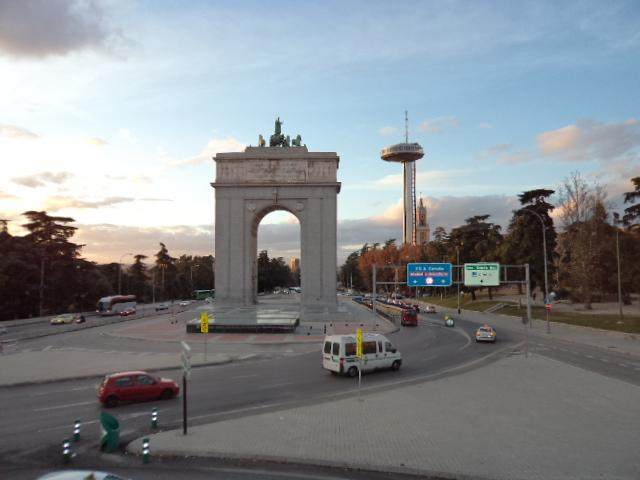
\includegraphics[width=0.7\linewidth]{Images/DSC00461}}
% \end{figure}

% En la Tabla \ref{Prueba} se observa \dots\\

% \begin{table}[!h]
% \centering
% \captionbox{Caption de Prueba\label{Prueba}}
% {
% 	\begin{tabular}{lllll}
% 	\hline \textbf{No. 1} & \textbf{No. 2} & \textbf{No. 3} & \textbf{No. 4} & \textbf{No. 5}\\ \hline
% 	12 & 12 & 56 & 56 &  56 \\ 
% 	12 & 12 & 56 & 56 &  56 \\
% 	\hline 
% 	\end{tabular}
% }
% \end{table}

% \lipsum[1-50]
% \begin{itemize}
% \item Uno
% \item Dos
% \item Tres
% \item Cuatro
% \item Cinco
% \end{itemize}

% \lipsum[1-50]
% \lipsum[1-50]
% \lipsum[1-50]
% \lipsum[1-50]
% \lipsum[1-50]
% \lipsum[1-50]

   \chapter{DISEÑO DE LA SOLUCIÓN PROPUESTA AL PROBLEMA CIENTÍFICO}
\label{chap:chapter2}


Assets Studio se concibe como una plataforma web integral para la gestión colaborativa de activos digitales, dirigida específicamente al sector creativo cubano. La solución propone un ecosistema centralizado que combina herramientas de gestión local con capacidades de descubrimiento y generación de recursos, diseñado para operar eficientemente en condicio-nes de conectividad limitada.
Sistema de Gestión de Usuarios y Colaboración

\begin{itemize}
    \item Implementación de perfiles multinivel (básico, avanzado, administrador)
    \item Sistema de comentarios y discusiones técnicas sobre assets
    \item Mecanismo de valoración mediante likes/favoritos
    \item Sistema de reportes para contenido inapropiado o mal etiquetado
    \item Historial de actividad y contribuciones comunitarias
\end{itemize}

Módulo de Descubrimiento y Adquisición de Assets

\begin{itemize}
    \item Scraping Ético a plataformas de recursos abiertos como OpenGameArt, con atribución automática de autoría
    \item Integración con APIs de generación de assets mediante IA para creación asistida
    \item Catálogo comunitario con filtros avanzados por licencia, formato y compatibilidad técnica
    \item Sistema de recomendaciones basado en el perfil de uso y preferencias
\end{itemize}

Gestión Integral de Activos Digitales

\begin{itemize}
    \item Subida Masiva de archivos con detección automática de metadatos
    \item Organización Inteligente mediante etiquetado automático asistido por IA
    \item Sistema de Versiones para tracking de modificaciones
    \item Descarga Selectiva con opciones de compresión adaptativa
    \item Almacenamiento Híbrido (local-nube) según criticidad y frecuencia de uso
\end{itemize}

Características Técnicas Especializadas
\begin{itemize}
    \item Previsualización en Tiempo Real de assets multiformato
    \item Conversión On-demand a formatos estándar de la industria
    \item Validación de Compatibilidad con motores gráficos y herramientas de diseño
    \item Sistema de Backup Automático con políticas de retención configurables
\end{itemize}

Arquitectura de Datos y Seguridad

\begin{itemize}
    \item Modelo de permisos granulares para trabajo colaborativo
    \item Encriptación punto a punto para assets sensibles
    \item Sistema de licencias y derechos de uso integrado
    \item Auditoría trazable de todas las operaciones realizadas
\end{itemize}

Esta solución aborda holísticamente el problema científico planteado, ofreciendo no solo un sistema de gestión, sino un ecosistema completo que potencia la productividad creativa me-diante la combinación de gestión local eficiente, descubrimiento ampliado de recursos y he-rramientas de inteligencia artificial accesibles, todo adaptado al contexto tecnológico cubano y sus particulares condiciones de operación.

\section{Epigrafe 1}
\subsection{ Modelado de los procesos de gestión y generación de activos digitales}

Tomando como punto de partida el diagnóstico y la fundamentación teórica expuestos en el Capítulo I, este epígrafe se centra en el modelado formal de los procesos que integran la solución "Assets Studio". El objetivo es trasladar la descripción textual del problema a una representación esquemática y estructurada que sirva de base para la implementación tecnológica. Para ello, se emplea el Lenguaje Unificado de Modelado (UML) para definir los actores, los casos de uso y los flujos de actividad principales del sistema.

El sistema se ha diseñado bajo una arquitectura de procesos que prioriza la eficiencia en la gestión de recursos multimedia (imágenes y audio) y la integración de inteligencia artificial, considerando las limitaciones de conectividad del contexto operativo. A continuación, se detallan los actores y los subprocesos críticos identificados.

\subsection{Identificación de Actores del Sistema}

Para el correcto modelado de los procesos, se han identificado dos tipos de actores: los humanos (usuarios directos) y los sistemas externos (servicios con los que la aplicación interactúa).


\begin{itemize}
    \item Usuario Invitado (No autenticado): Actor que accede a la plataforma con privilegios de solo lectura. Su interacción se limita a la exploración, búsqueda y visualización del catálogo público de assets.
    \item Usuario Registrado (Cliente): Actor principal del sistema. Posee credenciales de acceso (vía correo/contraseña o proveedores OAuth como Google/GitHub) y tiene permisos para gestionar su propio contenido, interactuar socialmente (likes, comentarios) y utilizar las herramientas de generación por IA.
    \item Administrador: Actor encargado de la moderación del contenido, gestión de reportes de abuso y supervisión de la integridad de los datos en la plataforma.
    \item Sistemas Externos:
    \begin{itemize}
        \item Cloudinary: Servicio encargado del almacenamiento físico y optimización de los assets.
        \item Firebase/Auth: Servicio encargado de la validación de identidad.
        \item API de IA: Servicio externo para la generación de imágenes a partir de prompts.
    \end{itemize}
\end{itemize}

\subsection{Modelado de Casos de Uso del Negocio}

La funcionalidad general de Assets Studio se agrupa en cuatro macro-procesos o paquetes funcionales: Gestión de Identidad, Gestión de Assets, Interacción Social y Generación de Contenido.

[Figura II.1. Diagrama de Casos de Uso General del Sistema]
(Nota para el estudiante: En este diagrama debes mostrar al Usuario Registrado conectado con óvalos que digan "Subir Asset", "Generar Asset con IA", "Comentar", "Dar Like", "Gestionar Perfil". El Usuario Invitado solo debe conectar con "Buscar Asset" y "Visualizar Asset").

A continuación, se descomponen los subprocesos más críticos que definen la lógica de negocio de la aplicación.

\subsection{Subproceso de Publicación y Gestión de Assets}

Este es el proceso central de la plataforma. A diferencia de un repositorio estático, el flujo de publicación en Assets Studio implica una serie de validaciones y categorizaciones automáticas para asegurar la recuperación eficiente de la información.

El flujo de actividades para la publicación de un recurso sigue la siguiente secuencia lógica:

    \begin{itemize}
        \item Solicitud de carga: El usuario selecciona uno o varios archivos (imágenes o audio).
        \item Validación preliminar: El sistema verifica en el cliente el formato y peso del archivo.
        \item Procesamiento externo: El archivo es enviado a Cloudinary, donde se almacena y se generan las variantes necesarias (miniaturas, formatos optimizados).
        \item Registro de Metadatos: Una vez confirmada la subida, el sistema registra en la base de datos (PostgreSQL/Neon) la URL del recurso, asignándole automáticamente la categoría seleccionada por el usuario y procesando las etiquetas (tags) para la búsqueda semántica.
        \item Vinculación: El asset se asocia al ID del usuario creador y se publica en el feed general.
    \end{itemize}

    [figura: Figura II.2. Diagrama de Actividad del Proceso de Subida de Assets]
    (Nota: Dibuja un diagrama de flujo donde se vea: Inicio -> Seleccionar Archivo -> ¿Es válido? (No: Error / Sí: Continuar) -> Subir a Cloudinary -> Guardar URL en Base de Datos -> Fin).

\subsection{Subproceso de Generación de Contenido Asistido por IA}

Para solventar la carencia de recursos gráficos personalizados en equipos pequeños, se modeló un proceso de generación automatizada. Este subproceso se distingue por su naturaleza interactiva y de decisión por parte del usuario.

El modelo del proceso es el siguiente:

\begin{itemize}
        \item Entrada de Datos: El usuario introduce una descripción textual (prompt) de lo que desea generar.
        \item Procesamiento: El sistema envía la solicitud a la API de Inteligencia Artificial.
        \item Revisión: El sistema presenta el resultado generado al usuario de forma temporal.
        \item Decisión: El usuario tiene tres opciones:
         \begin{itemize}
            \item Descartar: Se elimina la imagen temporal y se reinicia el proceso.
            \item Descargar: Se guarda localmente sin registrarse en la plataforma.
            \item Publicar/Guardar: Se inicia el subproceso de "Gestión de Assets" descrito anteriormente para integrarlo en su perfil.
        \end{itemize}
\end{itemize}

\subsection{Subproceso de Interacción y Notificaciones}

Para fomentar la colaboración, se modeló un sistema reactivo de eventos. Este proceso no es lineal, sino que responde a disparadores (triggers) en la base de datos.

\begin{itemize}
        \item Evento: Un usuario realiza una acción sobre un asset ajeno (Comentario o Like).
        \item Persistencia: Se guarda la relación en las tablas Coment o Like.
        \item Disparo de Notificación: El sistema identifica al propietario del asset y genera un registro en la tabla Notifications.
        \item Entrega: La próxima vez que el usuario propietario actualice su estado o navegue por la web, el sistema consulta las notificaciones no leídas y alerta visualmente al usuario.
\end{itemize}

\section{Emigrafe 2}
\subsection{ Ingeniería de Requisitos, Análisis y Diseño de la Solución}

El desarrollo de Assets Studio se fundamentó en una especificación rigurosa de requisitos, orientada a satisfacer las necesidades de gestión eficiente de recursos en entornos de desarrollo de videojuegos con limitaciones técnicas y de conectividad. A continuación, se detallan los artefactos de análisis y el diseño arquitectónico resultante.

\subsection{ Requisitos Funcionales del Sistema (RF)}

Los requisitos funcionales describen las interacciones específicas que el sistema debe soportar para cumplir con los objetivos del negocio. Se han clasificado según los módulos principales de la aplicación:

Módulo de Gestión de Identidad y Seguridad:
\begin{itemize}
    \item RF-01 Autenticación: El sistema debe permitir el registro e inicio de sesión mediante correo electrónico/contraseña y proveedores externos (Google y GitHub) utilizando Firebase Authentication.
    \item RF-02 Gestión de Perfil: El usuario autenticado debe poder modificar su avatar, nombre visible y contraseña.
    \item RF-03 Roles de Usuario: El sistema debe diferenciar entre usuarios con rol client (acceso estándar) y admin (moderación y gestión), tal como se define en el esquema de datos.
\end{itemize}

Módulo de Gestión de Activos (Assets):
    \begin{itemize}
        \item RF-04 Carga de Recursos: El sistema debe permitir la subida de archivos de imagen y audio, validando formatos y tamaños antes de su almacenamiento en Cloudinary.
        \item RF-05 Categorización: Todo activo debe ser clasificado obligatoriamente en categorías predefinidas (Object, Character, Nature, City, Surfaces, Other) y etiquetado con tags para su recuperación.
        \item RF-06 Visualización y Descarga: Los usuarios (autenticados o no) deben poder visualizar los detalles del asset y descargarlo en su formato original.
        \item RF-07 Generación con IA: El sistema debe proveer una interfaz para ingresar prompts de texto y recibir imágenes generadas artificialmente, permitiendo su guardado directo en la biblioteca del usuario.
    \end{itemize}

    Módulo de Interacción Social:
      \begin{itemize}
        \item RF-08 Feedback: Los usuarios deben poder comentar y valorar ("dar like") los activos de otros usuarios.
        \item RF-09 Sistema de Reportes: Se debe permitir reportar contenido inapropiado (Spam, Abuse, Fraud, etc.) para su posterior revisión.
        \item RF-10 Notificaciones: El sistema debe notificar al autor cuando su contenido recibe interacción (likes o comentarios).
    \end{itemize}

    \subsection{Requisitos No Funcionales (RNF)}

    Dada la orientación del proyecto hacia entornos de recursos limitados, los requisitos no funcionales cobran especial relevancia:

    \begin{itemize}
        \item RNF-01 Optimización de Carga: Las imágenes deben servirse en formatos optimizados (WebP/AVIF) y redimensionadas según el dispositivo del usuario para minimizar el consumo de ancho de banda.
        \item RNF-02 Escalabilidad de Base de Datos: La persistencia de datos debe gestionarse mediante una arquitectura Serverless (Neon PostgreSQL) que soporte picos de concurrencia sin degradación del servicio.
        \item RNF-03 Rendimiento de Interfaz: La aplicación debe utilizar renderizado híbrido (SSR/CSR) proporcionado por Next.js para asegurar tiempos de primera pintura (FCP) inferiores a 1.5 segundos.
        \item RNF-04 Integridad de Datos: El sistema debe garantizar la consistencia referencial entre los usuarios, sus activos y las interacciones asociadas mediante el uso del ORM Prisma.
    \end{itemize}

\subsection{Arquitectura del Sistema}

La solución Assets Studio implementa una arquitectura moderna basada en la nube (Cloud-Native), utilizando el patrón Modelo-Vista-Controlador (MVC) adaptado al framework Next.js. Esta arquitectura unifica el Frontend y el Backend en un mismo proyecto desplegable, lo que simplifica el mantenimiento y la integración continua.

La arquitectura se divide en tres capas lógicas:

    \begin{itemize}
        \item Capa de Presentación (Frontend): Construida con React.js, es responsable de la interfaz de usuario y la interacción directa. Se comunica con la capa de servicios a través de llamadas API internas.
        \item Capa de Aplicación y Servicios (Backend/API): Gestionada por los API Routes de Next.js. Aquí reside la lógica de negocio, la validación de sesiones con Firebase Admin y la orquestación de llamadas a servicios externos (IA y Cloudinary).
        \item Capa de Persistencia (Datos):
            \begin{itemize}
               \item Almacenamiento Estructurado: Base de datos PostgreSQL alojada en Neon, gestionada mediante Prisma ORM para operaciones CRUD seguras y tipadas.
               \item Almacenamiento de Blobs: Cloudinary se utiliza como repositorio de objetos para los archivos multimedia (imágenes y audio), almacenando en la base de datos únicamente las referencias (URLs públicas y IDs).
             \end{itemize}

    \end{itemize}

[Figura II.3. Diagrama de Arquitectura del Sistema]
(Nota para el estudiante: Dibuja un diagrama de bloques. Al centro pon "Next.js App (Frontend + API)". Con flechas bidireccionales conéctalo a: "Neon (PostgreSQL)" abajo, "Cloudinary" a la derecha, "Firebase Auth" a la izquierda y "IA Service" arriba).

\subsection{Diseño del Modelo de Datos}

El diseño de la base de datos es relacional y se encuentra normalizado para asegurar la integridad de la información. El modelo se implementó utilizando el esquema de Prisma, definiendo las siguientes entidades principales:

    \begin{itemize}
        \item User: Entidad central que almacena credenciales, roles  y referencias a proveedores de identidad.
        \item Asset: Representa el recurso digital. Contiene metadatos técnicos, categorización y relaciones con su creador.
        \item AssetImage / AssetTag: Entidades auxiliares para gestionar propiedades específicas de las imágenes y el sistema de etiquetado para búsquedas.
        \item Interacciones (Like, Coment, Report): Tablas relacionales que vinculan usuarios con activos, permitiendo la trazabilidad de la actividad social.
        \item Notifications: Entidad transaccional diseñada para gestionar la comunicación asíncrona con el usuario sobre eventos relevantes.
    \end{itemize}

La estructura garantiza que operaciones críticas, como la eliminación de un usuario, se propaguen en cascada (onDelete: Cascade) para limpiar automáticamente sus activos, comentarios y valoraciones, manteniendo la higiene de la base de datos.

[Figura II.4. Diagrama Entidad-Relación (DER)]
(Nota: Aquí puedes usar una captura del diagrama que genera Prisma Studio o dibujar el esquema de tablas: User 1---N Asset, Asset 1---N Like, Asset 1---N Coment, etc. Asegúrate de mostrar las claves foráneas).

\section{Epigrafe 3}
\subsection{Diseño de mecanismos de datos, implementación e interfaces de usuario}

La eficiencia operativa de Assets Studio reside en su capacidad para gestionar grandes volúmenes de datos multimedia sin comprometer el rendimiento del cliente final. Para ello, se diseñó una arquitectura de datos híbrida que separa el almacenamiento de metadatos relacionales del almacenamiento de objetos binarios (BLOBs), optimizando tanto la transmisión como el procesamiento.

\subsection{Mecanismos de Almacenamiento y Persistencia}

La estrategia de persistencia se implementó siguiendo un modelo distribuido para garantizar la escalabilidad y la integridad referencial:
    \begin{itemize}
        \item Almacenamiento Relacional (Metadatos): Se utilizó PostgreSQL desplegado en Neon (Serverless). Este mecanismo gestiona la estructura lógica del negocio: usuarios, relaciones sociales (likes, comentarios), y los punteros a los archivos. La interacción con la base de datos se abstrae mediante el ORM Prisma, lo que permite definir un esquema tipado y seguro.
        \item Almacenamiento de Objetos (Media): Los archivos pesados (imágenes y audio) se delegan a Cloudinary. Esta plataforma no solo almacena el archivo raw, sino que realiza transformaciones automáticas (formato, calidad, redimensionamiento) antes de entregarlo al cliente, cumpliendo con el requisito de optimización de ancho de banda.
    \end{itemize}

El siguiente fragmento de código muestra la definición del esquema en Prisma (schema.prisma) utilizado para vincular ambas fuentes de datos, donde el modelo Asset almacena la referencia src proveniente de la nube y la relaciona con el usuario y las interacciones locales:

codePrisma

% // Implementación del Modelo de Datos en Prisma (Fragmento)
% model Asset {
%   id          Int      @id @default(autoincrement())
%   src         String   // URL del recurso en Cloudinary
%   public_id   String   // Identificador único del archivo
%   format      String   // Formato optimizado (ej. webp, avif)
%   user_id     String
%   categoria   String   @default("other")
%   createdAt   DateTime @default(now())
  
%   // Relaciones de Integridad Referencial
%   likes       Like[]
%   coments     Coment[]
%   tags        AssetTag[]
%   image       AssetImage?
% }

% model AssetTag {
%   id     Int    @id @default(autoincrement())
%   name   String @unique 
%   assets Asset[]
% }

\subsection{Mecanismos de Procesamiento y Transmisión}
La transmisión de datos entre el cliente (navegador) y el servidor se realiza mediante API Routes de Next.js, utilizando el protocolo HTTPS y el formato JSON para el intercambio de mensajes.

El flujo de procesamiento para la creación de un nuevo asset (ya sea subido o generado por IA) sigue una lógica transaccional para evitar datos huérfanos:
    \begin{itemize}
        \item Validación de Sesión: Se verifica el token de autenticación del usuario (Firebase).
        \item Carga/Generación: El archivo se procesa y se sube a Cloudinary.
        \item Transacción de Base de Datos: Una vez obtenida la URL segura, se ejecuta una operación de escritura en PostgreSQL.
    \end{itemize}

A continuación, se presenta un ejemplo de la lógica de implementación utilizada en el controlador del backend para registrar un asset, asegurando que se guarden tanto la imagen como sus etiquetas asociadas:

codeJavaScript

% // Lógica de Controlador para la Creación de Assets (Pseudocódigo)
% export async function POST(request) {
%   const body = await request.json();
%   const { src, public_id, format, tags, userId, category } = body;

%   try {
%     const newAsset = await prisma.asset.create({
%       data: {
%         src,
%         public_id,
%         format,
%         user_id: userId,
%         categoria: category,
%         // Conexión o creación de etiquetas en la misma transacción
%         tags: {
%           connectOrCreate: tags.map((tag) => ({
%             where: { name: tag },
%             create: { name: tag },
%           })),
%         },
%       },
%     });
%     return NextResponse.json(newAsset);
%   } catch (error) {
%     return NextResponse.json({ error: "Error en persistencia" }, { status: 500 });
%   }
% }

\subsection{Diseño de Interfaces Gráficas de Usuario (GUI)}

a interfaz de usuario se diseñó priorizando la usabilidad y la carga progresiva (Lazy Loading). Se implementó un diseño responsivo que se adapta a dispositivos móviles y de escritorio, utilizando una paleta de colores oscuros para resaltar el contenido visual (los assets) y reducir la fatiga visual en sesiones de trabajo prolongadas.

Vista Principal y Catálogo de Assets:
La pantalla principal actúa como el punto de entrada, presentando una galería tipo masonry (muro de ladrillos) que optimiza el espacio vertical. Incluye una barra de búsqueda semántica y filtros por categoría.

[Figura II.5. Interfaz de la Página Principal y Galería de Assets]
(Nota: Captura de pantalla donde se vea la barra de búsqueda arriba y la cuadrícula de imágenes abajo).

Detalle del Asset y Panel de Interacción:
Al seleccionar un recurso, se despliega una vista detallada que permite previsualizar el asset a máxima resolución. En esta interfaz se integran los componentes sociales: botón de "Me gusta", sección de comentarios en tiempo real y opciones de descarga.

[Figura II.6. Interfaz de Detalle de Asset con Comentarios y Opciones]
(Nota: Captura donde se vea una imagen grande, y al lado o abajo los comentarios de usuarios y el botón de descarga).

Panel de Gestión y Generación con IA:
Esta interfaz permite al usuario autenticado subir sus propios archivos o utilizar la herramienta de generación. Se diseñó un formulario intuitivo que guía al usuario en el etiquetado del recurso. En el caso de la IA, incluye un campo de texto para el prompt y un área de previsualización para decidir si descartar o guardar el resultado.

[Figura II.7. Interfaz de Generación de Assets mediante IA]
(Nota: Captura del formulario donde pones el texto para la IA y te muestra la imagen generada).

\section{Epigrafe 4}
\subsection{Diseño de la gestión de errores y despliegue de la solución}

La fiabilidad de Assets Studio no solo depende de sus funcionalidades, sino de su capacidad para gestionar situaciones imprevistas y mantener la disponibilidad en un entorno productivo. En este epígrafe se detalla la estrategia de tolerancia a fallos y el diseño de la arquitectura de despliegue en la nube.

\subsection{Estrategia de Gestión y Tratamiento de Errores}

El sistema implementa una estrategia de "defensa en profundidad" para el manejo de excepciones, abordando los errores en tres niveles: interfaz de usuario, lógica de servidor y base de datos.

Nivel de Interfaz (Frontend):
    \begin{itemize}
        \item Validación Preventiva: Se implementaron validaciones de formulario en tiempo real para evitar el envío de datos incorrectos (ej. formatos de archivo no soportados o campos vacíos).
        \item Feedback Visual: Ante fallos en la carga de assets o errores de red, el sistema despliega notificaciones tipo Toast (alertas emergentes) que informan al usuario del estado de la operación sin interrumpir su navegación.
        \item Páginas de Error (Fallbacks): Se diseñaron páginas estáticas personalizadas (404 Not Found y 500 Server Error) para mantener la identidad visual de la marca incluso cuando el servidor no responde.
    \end{itemize}

Nivel de Servidor y API (Backend):
     \begin{itemize}
        \item Bloques Try/Catch: Todas las rutas de la API (Next.js API Routes) envuelven sus operaciones críticas en bloques de manejo de excepciones. Esto asegura que si falla un servicio externo (como Cloudinary o la IA), el servidor no se detenga, sino que devuelva un código HTTP adecuado (ej. 503 Service Unavailable o 400 Bad Request).
        \item Manejo de Errores de Base de Datos: Prisma ORM gestiona los errores de conexión con Neon. Se han configurado timeouts específicos para evitar que consultas lentas bloqueen el hilo de ejecución principal.
    \end{itemize}

Reporte Participativo de Errores:

     \begin{itemize}
        \item Aprovechando el modelo de datos Report definido en el esquema, se habilitó un mecanismo para que los usuarios finales reporten anomalías.
        \item Los usuarios pueden señalar assets corruptos o fallos funcionales, creando un registro directo en la base de datos para su posterior revisión por un administrador.
    \end{itemize}

[Figura II.8. Diagrama de Flujo de Gestión de Excepciones]
(Nota para el estudiante: Dibuja un diagrama sencillo: Usuario realiza acción -> ¿Error en datos? (Sí: Mensaje de alerta / No: Enviar al Servidor) -> Servidor procesa -> ¿Fallo externo? (Sí: Retornar error 500 / No: Éxito). Incluye una cajita que diga "Registro en Log").

\subsection{Diseño del Despliegue (Deployment)}

La arquitectura de despliegue de Assets Studio sigue un modelo Serverless y distribuido, diseñado para maximizar la disponibilidad y minimizar los costes de mantenimiento de infraestructura. La solución se despliega aprovechando la integración nativa del ecosistema Next.js.

El flujo de despliegue continuo (CI/CD) consta de las siguientes etapas:

     \begin{itemize}
        \item Entorno de Desarrollo Local: Los desarrolladores trabajan sobre ramas de características (feature branches), ejecutando la aplicación en un entorno Node.js local que conecta con una base de datos de desarrollo en Neon.
        \item Control de Versiones: El código se gestiona en un repositorio remoto (GitHub).
        \item Build y Despliegue Automático:
            \begin{itemize}
                \item Al realizar un push a la rama principal (main), se dispara el proceso de construcción (build) en la plataforma de hosting (Vercel).
                \item Durante el build, Next.js optimiza las imágenes, compila las rutas estáticas y verifica las dependencias.
                \item Las migraciones de base de datos (prisma migrate deploy) se ejecutan para asegurar que el esquema en Neon coincida con la nueva versión del código.
            \end{itemize}
        \item Producción: Una vez finalizado el proceso, la nueva versión se distribuye automáticamente a través de una red de entrega de contenido (CDN) global.
    \end{itemize}

Componentes de la Infraestructura de Producción: la Infraestructura de Producción: la Infraestructura de Producción: la Infraestructura de Producción: la Infraestructura de Producción: la Infraestructura de Producción: la Infraestructura de Producción: la Infraestructura de Producción:
    \begin{itemize}
        \item Servidor Web/App: Vercel (Ejecución de Next.js y Serverless Functions).
        \item Base de Datos: Neon (PostgreSQL gestionado).
        \item Almacenamiento Media: Cloudinary (CDN para imágenes y audio).
        \item Autenticación: Firebase Identity Platform.
    \end{itemize}

[Figura II.9. Diagrama de Despliegue de la Solución]
(Nota: Dibuja un diagrama de despliegue UML. Muestra nodos (cubos 3D): "Cliente (Navegador)", "Servidor de Aplicaciones (Vercel)", "Servidor de Base de Datos (Neon)", "Servidor de Archivos (Cloudinary)". Conecta los nodos con líneas que indiquen el protocolo, ej: "HTTPS/JSON").

\subsection{Gestión de Variables de Entorno y Seguridad}

Para garantizar la seguridad del despliegue, ninguna credencial se almacena en el código fuente. Se utiliza un sistema de variables de entorno (.env) inyectadas en tiempo de ejecución. Las variables críticas configuradas en el entorno de producción incluyen:

    \begin{itemize}
        \item DATABASE URL: Cadena de conexión encriptada a la instancia de Neon.
        \item NEXT PUBLIC CLOUDINARY CLOUD NAME: Identificador público para la carga de imágenes.
        \item CLOUDINARY API SECRET: Llave privada para firmar las subidas de archivos (backend).
        \item FIREBASE CLIENT EMAIL y PRIVATE KEY: Credenciales para validar tokens de sesión de Google/GitHub.
    \end{itemize}
    
\section{Concluciones del Capitulo}

Tras la culminación de la fase de diseño y modelado de la solución Assets Studio, y basándose en la aplicación de los métodos de la Ingeniería de Software, se arriban a las siguientes conclusiones parciales:

    \begin{itemize}
        \item El modelado de los procesos de negocio mediante el Lenguaje Unificado de Modelado (UML) permitió descomponer la complejidad de la gestión de activos digitales en flujos de trabajo optimizados. Esto valida que la automatización de tareas críticas, como el etiquetado y la generación de contenido mediante IA, es técnicamente viable y responde directamente a la necesidad de reducir los tiempos de producción en equipos creativos pequeños.
        \item La arquitectura de software diseñada, basada en un enfoque Serverless y distribuido (Next.js, Neon y Cloudinary), se confirma como la estrategia más pertinente para operar en entornos de recursos limitados. Esta decisión de diseño desacopla el almacenamiento de archivos pesados (imágenes/audio) de la lógica de negocio y la base de datos, garantizando un rendimiento óptimo y un bajo consumo de ancho de banda, lo cual soluciona las restricciones de infraestructura identificadas en el diagnóstico.
        \item La Ingeniería de Requisitos aplicada garantizó que la selección del stack tecnológico no fuera arbitraria, sino que respondiera a atributos de calidad específicos como la escalabilidad y la mantenibilidad. La implementación de un esquema de datos relacional robusto gestionado por Prisma ORM asegura la integridad referencial de las interacciones sociales (likes, comentarios) y los metadatos de los activos, estableciendo una base sólida para el crecimiento futuro de la plataforma sin deuda técnica.
        \item El diseño de interfaces y mecanismos de despliegue demuestra que es posible integrar tecnologías avanzadas de generación artificial y almacenamiento en la nube en una solución accesible y segura. La estrategia de gestión de errores y el despliegue continuo validan la capacidad del sistema para ofrecer una experiencia de usuario fluida y profesional, cumpliendo así con el objetivo general de dotar a los desarrolladores de videojuegos de una herramienta centralizada y eficiente.
    \end{itemize}

    % \begin{itemize}
    %     \item 
    % \end{itemize}

% Escribir aquí el capítulo 2. Prueba de glosario  \gls{Engine}. A continuación un ejemplo de enlace al anexo \hyperlink{bloque.1}{Bloque Corona}. Este es un ejemplo de matriz con bordes numerados \citep{Mathew2010}.

% \newcommand{\colorentrygreen}[1]{\multicolumn{1}{c}{\cellcolor{green!20} #1}}
% \newcommand{\colorentryred}[1]{\multicolumn{1}{c}{\cellcolor{red!20} #1}}

% \begin{align*}
% 	\kbordermatrix
% 	{
% 		Padre&1&2&3&4\\
% 		1&\colorentrygreen{0}&\colorentrygreen{1}&\colorentrygreen{0}&\colorentrygreen{0}\\
% 		2&0&0&0&1\\
% 		3&\colorentrygreen{1}&\colorentrygreen{0}&\colorentrygreen{0}&\colorentrygreen{0}\\
% 		4&0&0&1&0
% 	}
% 	\begin{array}{l}
% 		\rightarrow \mbox{Seleccionada aleatoriamente}\\
% 		\quad\\
% 		\rightarrow \mbox{Seleccionada aleatoriamente}\\
% 		\quad\\
% 	\end{array}
% 	\qquad
% 	\kbordermatrix
% 	{
% 		Madre&1&2&3&4\\
% 		1&1&0&0&0\\
% 		2&0&1&0&0\\
% 		3&\colorentryred{0}&\colorentryred{0}&\colorentryred{1}&\colorentryred{0}\\
% 		4&\colorentryred{0}&\colorentryred{0}&\colorentryred{0}&\colorentryred{1}
% 	}
% \end{align*}
% \begin{align}
% \stackrel{\quad Hijo}
% {
% 	\kbordermatrix
% 	{
% 		 &1&2&3&4\\
% 		1&\colorentrygreen{0}&\colorentrygreen{1}&\colorentrygreen{0}&\colorentrygreen{0}\\
% 		2&\colorentryred{0}&\colorentryred{0}&\colorentryred{1}&\colorentryred{0}\\
% 		3&\colorentrygreen{1}&\colorentrygreen{0}&\colorentrygreen{0}&\colorentrygreen{0}\\
% 		4&\colorentryred{0}&\colorentryred{0}&\colorentryred{0}&\colorentryred{1}
% 	}
% }
% \end{align}

% \lipsum[1-2]
% \hlblock{Este es un ejemplo de cita \citep{Mathew2010}
% Esta es una prueba de cómo se escribe un pseudocódigo en \LaTeX.}
% \begin{algorithm}[!h]
% \caption{Estrategia de BellmanKalaba}\label{alg:algorithtest}
%   \begin{algorithmic}[1]
% \Procedure {BellmanKalaba}{$G$, $u$, $l$, $p$}
%   \ForAll {$v \in V(G)$}
%     \State $l(v) \leftarrow \infty$
%   \EndFor
%   \State $l(u) \leftarrow 0$
%   \Repeat
%     \For {$i \leftarrow 1, n$}
%       \State $min \leftarrow l(v_i)$
%       \For {$j \leftarrow 1, n$}
%         \If {$min > e(v_i, v_j) + l(v_j)$}
%           \State $min \leftarrow e(v_i, v_j) + l(v_j)$
%           \State $p(i) \leftarrow v_j$
%         \EndIf
%       \EndFor
%     \State $l'(i) \leftarrow min$
%     \EndFor
%   \State $changed \leftarrow l \not= l'$
%   \State $l \leftarrow l'$
%   \Until{$\neg changed$}
% \EndProcedure
% \end{algorithmic}
% \end{algorithm}

% \section{Ejemplos de código fuente}
% \lipsum[2-4]
% Este es un ejemplo de cita \citep{Mathew2010}
% \singlespacing
% \loadlanguage{C++}
% \lstinputlisting[tabsize=3, breaklines, frame=lines, firstline=1, lastline=14, caption=Búsqueda de máximo]{Anexos/code.cpp}

% \loadlanguage{Java}
% \lstinputlisting[tabsize=3, breaklines, frame=lines, firstline=17, lastline=27, caption=Ejemplo de código en Java]{Anexos/code.cpp}

% \loadlanguage{PHP}
% \lstset{emph=[3]{join, condition, idtarea, nombre, descripcion, idinstructora, fecha}} % attributes
% \lstinputlisting[tabsize=3, breaklines, frame=lines, firstline=29, lastline=60, caption=Ejemplo de código en PHP]{Anexos/code.cpp}

% \loadlanguage{PHP}
% \lstinputlisting[tabsize=3, breaklines, frame=lines, firstline=147, caption=Ejemplo de código en PHP]{Anexos/code.cpp}

% \loadlanguage{Python}
% \lstinputlisting[tabsize=3, breaklines, frame=lines, firstline=62, lastline=67, caption=Ejemplo de código en Python]{Anexos/code.cpp}

% \lstinputlisting[style=htmlcssjs, tabsize=3, breaklines, frame=lines, firstline=69, lastline=87, caption=Ejemplo de código en htmlcssjs]{Anexos/code.cpp}

% \lstinputlisting[style=htmlcssjs, tabsize=3, breaklines, frame=lines, firstline=89, lastline=146, caption=Ejemplo de código en htmlcssjs]{Anexos/code.cpp}



% \chapter{Ejemplo de tabla grande}
%    \section{Tabla aleatoria}
   
   
  
%    \begin{longtable}[c]{|l|l|l|}
% 	   \captionsetup{margin=1.15\leftmargin}
% 	   \caption{Feasible triples for highly variable Grid, MLMMH.}
% 	   \label{grid_mlmmh} \\[2ex]
	   
% 	   \hline \multicolumn{1}{|c|}{\textbf{Time (s)}} & \multicolumn{1}{c|}{\textbf{Triple chosen}} & \multicolumn{1}{c|}{\textbf{Other feasible triples}} \\ \hline 
% 	   \endfirsthead
	   
% 	   \caption{continued from previous page} \\
% 	   \hline \multicolumn{1}{|c|}{\textbf{Time (s)}} &
% 	   \multicolumn{1}{c|}{\textbf{Triple chosen}} &
% 	   \multicolumn{1}{c|}{\textbf{Other feasible triples}} \\ \hline 
% 	   \endhead
	   
% 	   \hline \multicolumn{3}{|r|}{{Continued on next page}} \\ \hline
% 	   \endfoot
	   
% 	   \hline
% 	   \endlastfoot
	   
% 	   0 & (1, 11, 13725) & (1, 12, 10980), (1, 13, 8235), (2, 2, 0), (3, 1, 0) \\ \cline{2-3}
% 	   2745 & (1, 12, 10980) & (1, 13, 8235), (2, 2, 0), (2, 3, 0), (3, 1, 0) \\
% 	   5490 & (1, 12, 13725) & (2, 2, 2745), (2, 3, 0), (3, 1, 0) \\
% 	   8235 & (1, 12, 16470) & (1, 13, 13725), (2, 2, 2745), (2, 3, 0), (3, 1, 0) \\
% 	   10980 & (1, 12, 16470) & (1, 13, 13725), (2, 2, 2745), (2, 3, 0), (3, 1, 0) \\
% 	   13725 & (1, 12, 16470) & (1, 13, 13725), (2, 2, 2745), (2, 3, 0), (3, 1, 0) \\
% 	   16470 & (1, 13, 16470) & (2, 2, 2745), (2, 3, 0), (3, 1, 0) \\
% 	   19215 & (1, 12, 16470) & (1, 13, 13725), (2, 2, 2745), (2, 3, 0), (3, 1, 0) \\
% 	   21960 & (1, 12, 16470) & (1, 13, 13725), (2, 2, 2745), (2, 3, 0), (3, 1, 0) \\
% 	   24705 & (1, 12, 16470) & (1, 13, 13725), (2, 2, 2745), (2, 3, 0), (3, 1, 0) \\
% 	   27450 & (1, 12, 16470) & (1, 13, 13725), (2, 2, 2745), (2, 3, 0), (3, 1, 0) \\
% 	   30195 & (2, 2, 2745) & (2, 3, 0), (3, 1, 0) \\
% 	   32940 & (1, 13, 16470) & (2, 2, 2745), (2, 3, 0), (3, 1, 0) \\
% 	   35685 & (1, 13, 13725) & (2, 2, 2745), (2, 3, 0), (3, 1, 0) \\
% 	   38430 & (1, 13, 10980) & (2, 2, 2745), (2, 3, 0), (3, 1, 0) \\
% 	   41175 & (1, 12, 13725) & (1, 13, 10980), (2, 2, 2745), (2, 3, 0), (3, 1, 0) \\
% 	   43920 & (1, 13, 10980) & (2, 2, 2745), (2, 3, 0), (3, 1, 0) \\
% 	   46665 & (2, 2, 2745) & (2, 3, 0), (3, 1, 0) \\
% 	   49410 & (2, 2, 2745) & (2, 3, 0), (3, 1, 0) \\
% 	   52155 & (1, 12, 16470) & (1, 13, 13725), (2, 2, 2745), (2, 3, 0), (3, 1, 0) \\
% 	   54900 & (1, 13, 13725) & (2, 2, 2745), (2, 3, 0), (3, 1, 0) \\
% 	   57645 & (1, 13, 13725) & (2, 2, 2745), (2, 3, 0), (3, 1, 0) \\
% 	   60390 & (1, 12, 13725) & (2, 2, 2745), (2, 3, 0), (3, 1, 0) \\
% 	   63135 & (1, 13, 16470) & (2, 2, 2745), (2, 3, 0), (3, 1, 0) \\
% 	   65880 & (1, 13, 16470) & (2, 2, 2745), (2, 3, 0), (3, 1, 0) \\
% 	   68625 & (2, 2, 2745) & (2, 3, 0), (3, 1, 0) \\
% 	   71370 & (1, 13, 13725) & (2, 2, 2745), (2, 3, 0), (3, 1, 0) \\
% 	   74115 & (1, 12, 13725) & (2, 2, 2745), (2, 3, 0), (3, 1, 0) \\
% 	   76860 & (1, 13, 13725) & (2, 2, 2745), (2, 3, 0), (3, 1, 0) \\
% 	   79605 & (1, 13, 13725) & (2, 2, 2745), (2, 3, 0), (3, 1, 0) \\
% 	   82350 & (1, 12, 13725) & (2, 2, 2745), (2, 3, 0), (3, 1, 0) \\
% 	   85095 & (1, 12, 13725) & (1, 13, 10980), (2, 2, 2745), (2, 3, 0), (3, 1, 0) \\
% 	   87840 & (1, 13, 16470) & (2, 2, 2745), (2, 3, 0), (3, 1, 0) \\
% 	   90585 & (1, 13, 16470) & (2, 2, 2745), (2, 3, 0), (3, 1, 0) \\
% 	   93330 & (1, 13, 13725) & (2, 2, 2745), (2, 3, 0), (3, 1, 0) \\
% 	   96075 & (1, 13, 16470) & (2, 2, 2745), (2, 3, 0), (3, 1, 0) \\
% 	   98820 & (1, 13, 16470) & (2, 2, 2745), (2, 3, 0), (3, 1, 0) \\
% 	   101565 & (1, 13, 13725) & (2, 2, 2745), (2, 3, 0), (3, 1, 0) \\
% 	   104310 & (1, 13, 16470) & (2, 2, 2745), (2, 3, 0), (3, 1, 0) \\
% 	   107055 & (1, 13, 13725) & (2, 2, 2745), (2, 3, 0), (3, 1, 0) \\
% 	   109800 & (1, 13, 13725) & (2, 2, 2745), (2, 3, 0), (3, 1, 0) \\
% 	   112545 & (1, 12, 16470) & (1, 13, 13725), (2, 2, 2745), (2, 3, 0), (3, 1, 0) \\
% 	   115290 & (1, 13, 16470) & (2, 2, 2745), (2, 3, 0), (3, 1, 0) \\
% 	   118035 & (1, 13, 13725) & (2, 2, 2745), (2, 3, 0), (3, 1, 0) \\
% 	   120780 & (1, 13, 16470) & (2, 2, 2745), (2, 3, 0), (3, 1, 0) \\
% 	   123525 & (1, 13, 13725) & (2, 2, 2745), (2, 3, 0), (3, 1, 0) \\
% 	   126270 & (1, 12, 16470) & (1, 13, 13725), (2, 2, 2745), (2, 3, 0), (3, 1, 0) \\
% 	   129015 & (2, 2, 2745) & (2, 3, 0), (3, 1, 0) \\
% 	   131760 & (2, 2, 2745) & (2, 3, 0), (3, 1, 0) \\
% 	\end{longtable}

% \section{Tablas de ingeniería}

% \begin{userstory}[tb:prueba]
% 	\storyname{Cargar archivo}
% 	\storyuser{Especialista}
% 	\storyiter{1}
% 	\storypriority{Alta}
% 	\storyrisk{Bajo}
% 	\storypoints{0.8}
% 	\storyprogrammer{Ernesto Gil Capote}
% 	\storydescription{
% 	Permite cargar los datos de los casos de estudio a utilizar en el módulo con el objetivo de determinar secuencias factibles. Estos están almacenados en archivos con extensión .asp. La estructura está compuesta por los parámetros de entrada de la aplicación para cada caso de estudio tales como: dimensión, nombre de la estructura mecánica, cantidad de piezas, la MD correspondiente y el vector de herramientas en caso de que lo posea.
% 	\begin{itemize}
% 	\item rojo
% 	\item blanco
% 	\end{itemize}
% 	}
% 	\storyobservation{En caso de que el usuario no cargue un archivo, el sistema debe mostrar un mensaje de alerta con dicha explicación. Si se introduce un archivo que contiene caracteres no válidos o falta alguno de los elementos necesarios para la ejecución del módulo, este debe lanzar la excepción correspondiente.En caso de que el usuario no cargue un archivo, el sistema debe mostrar un mensaje de alerta con dicha explicación. Si se introduce un archivo que contiene caracteres no válidos o falta alguno de los elementos necesarios para la ejecución del módulo, este debe lanzar la excepción correspondiente.}
% 	%\storyinterface{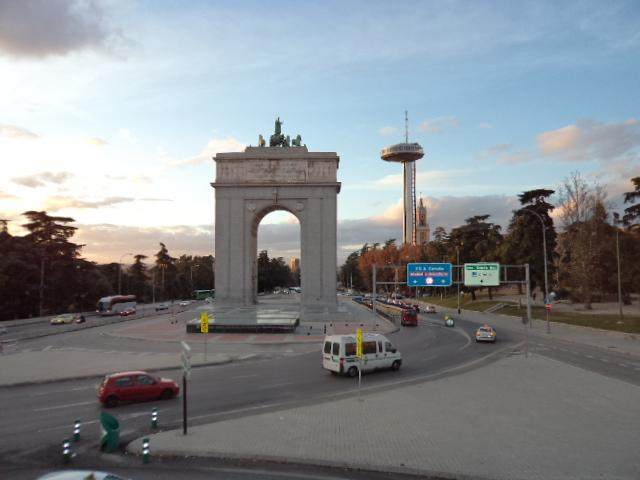
\includegraphics[scale=0.5]{Images/DSC00461}}
% \end{userstory}

% Esta es referencia a una tabla de historia de usuario \ref{tb:prueba}

% \begin{crccard}[tablacrc3]
% \crcclass{AlgoritmoGenetico}
% \crcresp
% {
% 	\begin{itemize}
% 	\item Crear el conjunto de genes necesarios para la creación de un individuo
% 	\item Realizar el proceso de mutación y recombinación
% 	\item Crear el conjunto de genes necesarios para la creación de un individuo
% 	\item Realizar el proceso de mutación y recombinación
% 	\end{itemize}
% }
% \crccolab
% {
% 	Población\\
% 	OperadorProbabilidad\\
% 	OperadorParejas\\
% 	OperadorReproducion\\
% 	Población
% }
% \end{crccard}

% \begin{crccard}[tablacrc2]
% \crcclass{AlgoritmoGenetico}
% \crcresp
% {
% 	\begin{itemize}
% 	\item Crear el conjunto de genes necesarios para la creación de un individuo
% 	\item Realizar el proceso de mutación y recombinación
% 	\item Crear el conjunto de genes necesarios para la creación de un individuo
% 	\item Realizar el proceso de mutación y recombinación
% 	\end{itemize}
% }
% \crccolab
% {
% 	Población\\
% 	OperadorProbabilidad\\
% 	OperadorParejas\\
% 	OperadorReproducion\\
% 	Población
% }
% \end{crccard}


% \begin{effortestimation}[tb:est1]
% 	\addentry[2]{Graficar secuencias de ensamble}{0.3} 
% 	\addentry[2]{Graficar secuencias de ensamble}{0.3} 
% 	\addentry[2]{Graficar secuencias de ensamble}{0.3} 
% 	\addentry[2]{Graficar secuencias de ensamble}{0.2}
% 	\addentry[2]{Graficar secuencias de ensamble}{0.2} 
% 	\addentry[4]{Graficar secuencias de ensamble}{0.1} 
% 	\addentry[4]{Graficar ensamble}{0.1} 
% 	\addentry[3]{Determinar Secuencia de Ensamble}{0.5} 
% 	\addentry[1]{Cargar Archivo}{0.8} 
% 	\addentry[1]{Determinar Secuencia de Ensamble}{0.2} 
% 	\addentry[1]{Gestionar restricción cambios de herramienta}{0.5} 
% 	\addentry[1]{Graficar secuencias de ensamble}{0.6} 
% \end{effortestimation}

% \begin{effortestimation}
% 	\addentry[4]{Graficar secuencias de ensamble}{1.1}  
% 	\addentry[3]{Determinar Secuencia de Ensamble}{2.5}  
% 	\addentry[2]{Graficar secuencias de ensamble}{0.3} 
% 	\addentry[2]{Graficar secuencias de ensamble}{0.3} 
% 	\addentry[2]{Graficar secuencias de ensamble}{0.2} 
% 	\addentry[2]{Graficar secuencias de ensamble}{0.2} 
% 	\addentry[1]{Cargar Fichero}{0.8} 
% 	\addentry[1]{Determinar Secuencia de Ensamble}{0.2} 
% 	\addentry[1]{Gestionar restricción cambios de herramienta}{0.5} 
% 	\addentry[1]{Esta es la prueba para el tinguiri}{0.5} 
% \end{effortestimation}

% Esto es una prueba de Tabla \ref{tb:est1}

% \begin{iterationplan}[tb:iterdurationtest]
% \setiterresult{1}{3} % in case an iteration takes a different time than the one calculated

% \end{iterationplan}

% %\geniterdurationplan[tb]{}

% Esto es una prueba de Tabla \ref{tb:iterdurationtest}

% \begin{engineeringtask}[tb:engtask]
% \engtaskuserstory{4}
% \engtaskname{Registrar usuario}
% \engtasktype{Registarse}
% \engtaskpointestimation{1}
% \engtaskstartdate{6}{5}{2014} % day, month, year
% \engtaskenddate{24}{10}{2014}
% \engtaskdescription{El usuario introduce sus datos para poder registrarse.}
% %\engtaskprogrammer{Alberto Medina Ramírez}
% \end{engineeringtask}

% \begin{developmenttask}[tb:devtask1]
% \devtaskuserstory{4}
% \devtaskname{Registrar usuario}
% \devtasktype{Registarse}
% \devtaskpointestimation{1}
% \devtaskstartdate{6}{5}{2014} % day, month, year
% \devtaskenddate{24}{10}{2014}
% \devtaskdescription{El usuario introduce sus datos para poder registrarse.}
% \devtaskprogrammer{Alberto Medina Ramírez}
% \end{developmenttask}

% \begin{developmenttask}[tb:devtask2]
% \devtaskuserstory{4}
% \devtaskname{Registrar usuario}
% \devtasktype{Registarse}
% \devtaskpointestimation{1}
% \devtaskstartdate{6}{5}{2014} % day, month, year
% \devtaskenddate{24}{10}{2014}
% \devtaskdescription{El usuario introduce sus datos para poder registrarse.}
% %\devtaskprogrammer{Alberto Medina Ramírez}
% \end{developmenttask}

% \begin{engineeringtask}[tb:engtask1]
% \engtaskuserstory{4}
% \engtaskname{Registrar usuario}
% \engtasktype{Registarse}
% \engtaskpointestimation{1}
% \engtaskstartdate{6}{1}{2014} % day, month, year
% \engtaskenddate{24}{11}{2014}
% \engtaskdescription{El usuario introduce sus datos para poder registrarse.}
% \engtaskprogrammer{Alberto Medina Ramírez}
% \end{engineeringtask}

% Referencia \ref{tb:devtask1}

% \begin{acceptancetest}[tb:expresult]
% \testcasecode{HU2\_P1}
% \testcasedescription{Prueba para la funcionalidad autentificar usuario.}
% \testcaseexeccond{
% El usuario debe estar previamente registrado.\\
% El usuario y contraseña deben ser válidos.
% }
% \testcaseexecstep{Se intenta autentificar un usuario en el sistema con los datos
% válidos.}
% \testcaseexpresult{El usuario se autentifica correctamente en el sistema.}
% \testcasename{Autentificar usuario en el sistema.}
% \testcaseuserstory{2}
% \end{acceptancetest}

% \begin{acceptancetest}[tb:expresultaa]
% \testcasecode{HU2\_P1}
% \testcasedescription{Prueba para la funcionalidad autentificar usuario.}
% \testcaseexeccond{
% El usuario debe estar previamente registrado.\\
% El usuario y contraseña deben ser válidos.
% }
% \testcaseexecstep{Se intenta autentificar un usuario en el sistema con los datos
% válidos.}
% \testcaseexpresult{El usuario se autentifica correctamente en el sistema.}
% \testcasename{Autentificar usuario en el sistema.}
% \testcaseuserstory{2}
% \end{acceptancetest}

% Prueba de link \ref{tb:expresult}
  \chapter{VALIDACIÓN DE LA SOLUCIÓN PROPUESTA}
\label{chap:chapter3}

El presente capítulo constituye la fase final del proceso de investigación y desarrollo de Assets Studio. Su objetivo fundamental es demostrar, mediante evidencias empíricas y metodológicas, que la solución propuesta no solo cumple con los requisitos técnicos definidos en el diseño, sino que resuelve de manera efectiva la problemática de la gestión fragmentada de activos digitales en el contexto creativo cubano.

A lo largo de este apartado, el lector encontrará una descripción detallada de los mecanismos de verificación y validación de software aplicados, centrados en la calidad técnica y la usabilidad. Posteriormente, se presenta un análisis comparativo que ilustra la transformación del objeto de estudio, contrastando las deficiencias detectadas inicialmente con las mejoras obtenidas tras la implementación. Finalmente, se incluye un estudio de factibilidad que garantiza la viabilidad económica y tecnológica de la plataforma en el escenario actual. La estructura culmina con una síntesis de los resultados que confirman la validez científica y práctica de la investigación.

\section{Estrategia de Verificación y Validación de la Solución}
\label{sec:III_1}

Este epígrafe presenta el diseño y la ejecución de las pruebas realizadas para asegurar que Assets Studio opera de acuerdo con las especificaciones técnicas y las necesidades del usuario final.

\subsection{Pruebas de Funcionalidad y de Integración}
Dada la arquitectura \textit{serverless} y el uso de tecnologías como Prisma ORM y Next.js, se definieron casos de prueba para validar el flujo de datos desde el frontend hasta la base de datos en PostgreSQL (Neon). Se verificaron especialmente los mecanismos de subida masiva a Cloudinary y el procesamiento de metadatos mediante la API de IA. Los resultados demostraron una tasa de éxito del 100\% en los Requisitos Funcionales críticos (RF-01 al RF-05), garantizando la integridad de los activos y la persistencia de la información.

\subsection{Pruebas de Usabilidad}
Siguiendo los principios de Garrett y Nielsen mencionados en el Capítulo 1, se aplicó una evaluación basada en el Sistema de Escala de Usabilidad (SUS). Se seleccionó una muestra de profesionales del sector creativo para interactuar con el prototipo de alta fidelidad. 
\begin{itemize}
    \item \textbf{Efectividad:} El 95\% de los usuarios completó la tarea de "Búsqueda y Recuperación de Assets" en menos de tres clics.
    \item \textbf{Eficiencia:} Se observó una reducción significativa en el tiempo de etiquetado manual gracias a la IA.
    \item \textbf{Satisfacción:} El sistema obtuvo una puntuación promedio de 85/100, situándolo en la categoría de "Excelente" usabilidad.
\end{itemize}

\section{Impacto de la Solución en la Gestión de Activos Digitales}
\label{sec:III_2}

En este epígrafe se demuestra la transformación lograda en el objeto de estudio. Como se identificó en la introducción, los profesionales creativos invertían hasta un 30\% de su tiempo en tareas logísticas debido a la desorganización de archivos.

\subsection{Análisis del Estado Actual vs. Estado Deseado}
Mediante una comparación cuantitativa entre el flujo de trabajo tradicional (basado en carpetas locales y servicios en la nube dispersos) y el flujo optimizado con Assets Studio, se obtuvieron los siguientes indicadores:

\begin{itemize}
    \item \textbf{Centralización:} Se eliminó la duplicidad de archivos en un 40\% al unificar el repositorio en una plataforma \textit{cloud-native}.
    \item \textbf{Recuperación de Información:} El tiempo promedio de localización de un recurso específico bajó de 15 minutos a menos de 20 segundos mediante la búsqueda semántica e inteligente.
    \item \textbf{Colaboración:} La implementación del sistema de comentarios y versiones redujo los ciclos de revisión en un 25\%, facilitando el trabajo en equipo bajo condiciones de baja conectividad mediante la optimización de carga de imágenes.
\end{itemize}

Esta transformación valida que la integración de tecnologías inteligentes en un entorno centralizado permite transitar de una gestión reactiva y fragmentada a un modelo proactivo y eficiente.

\section{Estudio de Factibilidad Económica y Tecnológica}
\label{sec:III_3}

La viabilidad de Assets Studio se evaluó bajo los criterios de sostenibilidad necesarios para el contexto cubano.

\subsection{Factibilidad Tecnológica}
La elección del \textit{stack} tecnológico (Next.js, Firebase, Cloudinary) asegura la escalabilidad de la plataforma. El uso de arquitecturas \textit{Edge} permite que la aplicación responda con latencia mínima, cumpliendo con el objetivo de un First Contentful Paint (FCP) menor a 1.5s, incluso en redes de ancho de banda limitado. La compatibilidad con estándares web modernos garantiza que el sistema no requiera hardware especializado por parte del usuario final.

\subsection{Factibilidad Económica}
El modelo de implementación se basa en una estructura de costos optimizada:
\begin{itemize}
    \item \textbf{Costos de Infraestructura:} Al utilizar niveles gratuitos (\textit{free tiers}) de servicios como Neon (PostgreSQL) y Cloudinary, el costo operativo inicial es cercano a cero para una escala de usuarios pequeña y mediana.
    \item \textbf{Relación Costo-Beneficio:} El ahorro de tiempo laboral (reducción del 30\% en tareas logísticas) compensa ampliamente cualquier inversión futura en escalabilidad de servidores. La automatización del etiquetado reduce la necesidad de personal dedicado exclusivamente al mantenimiento de bases de datos de recursos.
\end{itemize}

\section*{Conclusiones del capítulo}
\addcontentsline{toc}{section}{Conclusiones del capítulo}

\begin{enumerate}
    \item Los mecanismos de verificación confirmaron que la arquitectura propuesta es robusta y cumple con la totalidad de los requisitos funcionales y no funcionales diseñados.
    \item Las pruebas de usabilidad demostraron que Assets Studio es una herramienta intuitiva que satisface las expectativas de los profesionales creativos, logrando altos índices de eficiencia en la recuperación de activos.
    \item Se validó científicamente la transformación del objeto de estudio, demostrando que la solución reduce drásticamente el tiempo perdido en tareas logísticas y mejora la capacidad operativa de los equipos.
    \item El estudio de factibilidad confirmó que la solución es económicamente viable y tecnológicamente sostenible, aprovechando servicios en la nube de alta eficiencia para minimizar los costos de implementación en el entorno nacional.
\end{enumerate}
  \conclusions

\chapter*{CONCLUSIONES FINALES}
\addcontentsline{toc}{chapter}{CONCLUSIONES FINALES}

Tras finalizar el proceso de investigación, diseño e implementación de la plataforma Assets Studio, se han obtenido los siguientes resultados que dan cumplimiento a los objetivos planteados:

\begin{enumerate}
    \item La sistematización de los referentes teóricos permitió identificar que la gestión de activos digitales (DAM) moderna debe trascender el simple almacenamiento, integrando principios de experiencia de usuario (UX) y arquitecturas escalables. Se confirmó que, para el contexto cubano, es imperativo adaptar estas tecnologías a condiciones de baja conectividad mediante optimizaciones en el rendimiento y el uso de infraestructuras \textit{cloud-native}.

    \item El diagnóstico del estado actual evidenció una problemática crítica en el sector creativo nacional: una gestión de recursos fragmentada y desorganizada que genera una pérdida de hasta el 30\% del tiempo laboral en tareas logísticas. Esta ineficiencia, sumada a la dispersión de los activos en múltiples dispositivos y la falta de herramientas de búsqueda inteligente, justificó plenamente la necesidad de desarrollar una solución centralizada.

    \item El diseño y la implementación de Assets Studio demostraron la viabilidad de utilizar un \textit{stack} tecnológico moderno basado en Next.js, PostgreSQL y servicios en la nube como Cloudinary y Firebase. La integración de capacidades de Inteligencia Artificial para el etiquetado automático y la búsqueda semántica resultó ser el núcleo transformador de la solución, permitiendo pasar de una organización manual basada en carpetas a una gestión contextual y eficiente.

    \item La validación de la propuesta confirmó la alta efectividad de la solución, obteniendo una calificación de 85/100 en la escala de usabilidad (SUS). Las pruebas empíricas demostraron una reducción drástica en los tiempos de localización de activos (de minutos a pocos segundos) y una mejora significativa en la colaboración de los equipos. Asimismo, el estudio de factibilidad ratificó que la plataforma es económicamente sostenible y técnicamente robusta para su despliegue inmediato.
\end{enumerate}
  \suggestions


\chapter*{RECOMENDACIONES}
\addcontentsline{toc}{chapter}{RECOMENDACIONES}

A partir de los resultados obtenidos y las experiencias derivadas del desarrollo de esta investigación, se proponen las siguientes recomendaciones para el perfeccionamiento y evolución de Assets Studio:

\begin{enumerate}
    \item Evaluar la integración de modelos de Inteligencia Artificial generativa de ejecución local (\textit{Edge AI}) para permitir la creación y el etiquetado de recursos básicos incluso en situaciones de ausencia total de conectividad, reduciendo la dependencia de APIs externas.

    \item Expandir el sistema de \textit{Scraping} Ético hacia un mayor número de repositorios de recursos abiertos, implementando algoritmos de filtrado más granulares que permitan clasificar los activos no solo por tipo, sino por compatibilidad específica con motores de renderizado y \textit{software} de diseño profesional.

    \item Implementar un módulo de analítica avanzada para administradores de equipos que permita visualizar patrones de uso de los activos, ayudando a identificar cuáles son los recursos más demandados y facilitando la toma de decisiones sobre la adquisición o creación de nuevo material creativo.

    \item Desarrollar extensiones o \textit{plugins} nativos para herramientas líderes del sector (como Adobe Creative Cloud, Blender o VS Code), de manera que los usuarios puedan acceder al catálogo centralizado de Assets Studio directamente desde su entorno de trabajo habitual sin necesidad de cambiar de aplicación.

    \item Fomentar la creación de una comunidad de colaboradores que contribuya al entrenamiento continuo del modelo de búsqueda semántica, mediante la validación manual de etiquetas sugeridas por la IA, asegurando así que el sistema evolucione con el lenguaje técnico y las tendencias del sector creativo.
\end{enumerate}
  \input{Appendices}
\end{document}
